\section{Jリーグの営業支出}\label{s1:Jリーグの営業支出} %{
	\lstset{basicstyle=\ttfamily\small, language=R}
	Jリーグは各チームの収支報告を公開している。(PDF配布\cite{html:j-club})
	この資料の中で、2007-2008、2008-2009, 2009-2010年度の営業支出の分布を
	調べてみた。営業支出は人件費などのチーム運営に要する費用である。
	支出額と支出順位の関係を最小二乗法で近似した結果は次のようになった。
	(出力\ref{code:Jリーグの営業支出}と図\ref{fig:Jリーグの営業支出})
	\begin{equation*}\begin{split} %{
		(\text{支出額}) = (\text{支出順位})^{-\beta}e^{-\gamma(\text{支出順位})}
	\end{split}\end{equation*} %}
	ここで、$\beta$と$\gamma$は一部リーグJ1か二部リーグJ2かで異なる正の値で
	ある。Jリーグの場合、べき乗則$\beta$よりも指数ダンピング$\gamma$方が
	支配的になっている。Jリーグが主要な娯楽になっていないことが要因かも
	しれない。他国の状況も知りたいところだが、Jリーグのように各チームの
	経済状況を公開しているリーグを他に知らない。

	\begin{lstlisting}[caption=Jリーグの営業支出, label=code:Jリーグの営業支出]
Call:
lm(formula = log(budget) ~ league * (log(rank) + rank))

Residuals:
     Min       1Q   Median       3Q      Max 
-0.45610 -0.08077  0.02437  0.08866  0.29798 

Coefficients:
                    Estimate Std. Error t value Pr(>|t|)    
(Intercept)         8.692572   0.060908 142.717  < 2e-16 ***
leagueJ2            2.529275   1.563122   1.618   0.1090    
log(rank)          -0.134530   0.061011  -2.205   0.0299 *  
rank               -0.035883   0.008394  -4.275 4.59e-05 ***
leagueJ2:log(rank) -0.681790   0.722460  -0.944   0.3477    
leagueJ2:rank      -0.033228   0.031024  -1.071   0.2869    
---
Signif. codes:  0 ‘***’ 0.001 ‘**’ 0.01 ‘*’ 0.05 ‘.’ 0.1 ‘ ’ 1 

Residual standard error: 0.1397 on 94 degrees of freedom
Multiple R-squared: 0.9697,     Adjusted R-squared: 0.9681 
F-statistic: 602.1 on 5 and 94 DF,  p-value: < 2.2e-16
	\end{lstlisting}

	\begin{figure}[htbp] %{
		\begin{center}
			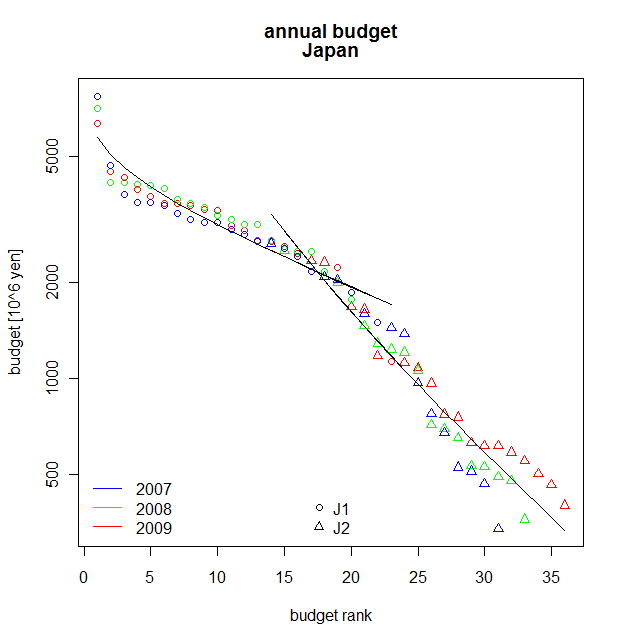
\includegraphics{fig/japan-budget.png}
		\end{center}
		\caption{Jリーグの営業支出}\label{fig:Jリーグの営業支出}
	\end{figure} %}
%s1:Jリーグの営業支出}

\section{スペインリーグの予算}\label{s1:スペインリーグの予算} %{
	Webでサッカーのスペインリーグでの予算(表\ref{tab:スペインリーグでの予算})
	が掲載されていたので、予算の分布と予算と成績との関係を調べてみた。
	\begin{equation*}\begin{array}{rcrcrl} %{
		\ln(\text{予算額}) &=& 6.2884 &-& 1.0953 & \ln(\text{予算順位}) \\
		\ln(\text{予算額}) &=& 5.9715 &-& 0.9397 & \ln(\text{リーグ戦順位}) \\
		\text{得点} &=& -14.223 &+& 8.996 & \ln(\text{予算額}) \\
		\ln(\text{失点}) &=& 4.00974 &-& 0.24946\ & \ln(\text{予算額}) \\
	\end{array}\end{equation*} %}
	予算額の値はちょっと嘘くさいと思う。このデータからほぼ
	\begin{equation*}\begin{split} %{
		\text{チームの予算額}
			=\frac{\text{予算順位一位の予算額}}{\text{チームの予算順位}}
	\end{split}\end{equation*} %}
	という関係が成り立つことになるが、あまりにもデータの値が揃いすぎている。
	普通に考えるともっとデータの値にばらつきがあると思う。

\begin{table}[!htbp]
\begin{center}
\begin{tabular}{rlrrrr} \hline
& チーム & 予算 [$10^6$ euro] & リーグ戦順位 & 得点 & 失点 \\ \hline
1 & Barcelona & 428.00 &   1 &  51 &   9 \\ 
2 & RealMadrid & 442.00 &   2 &  39 &  12 \\ 
3 & Villareal & 67.00 &   3 &  30 &  14 \\ 
4 & Valencia & 131.00 &   4 &  24 &  19 \\ 
5 & Espanol & 50.00 &   5 &  18 &  22 \\ 
6 & AtleticoMadrid & 110.00 &   6 &  27 &  19 \\ 
7 & Getafe & 24.00 &   7 &  27 &  19 \\ 
8 & AthleticBilbao & 53.10 &   8 &  25 &  27 \\ 
9 & RealSociedad & 35.00 &   9 &  22 &  26 \\ 
10 & Mallorca & 36.00 &  10 &  16 &  20 \\ 
11 & Sevilla & 90.00 &  11 &  21 &  27 \\ 
12 & Hercules & 42.00 &  12 &  18 &  22 \\ 
13 & Deportivo & 65.00 &  13 &  13 &  19 \\ 
14 & Racing & 42.00 &  14 &  13 &  23 \\ 
15 & Osasuna & 28.90 &  15 &  15 &  20 \\ 
16 & Levante & 20.00 &  16 &  18 &  26 \\ 
17 & Almeria & 28.00 &  17 &  15 &  25 \\
18 & Malaga &  &  18 &  20 &  35 \\ 
19 & Sporting & 25.00 &  19 &  12 &  23 \\ 
20 & Zaragoza & 24.50 &  20 &  13 &  26 \\ \hline
\end{tabular}
\caption{スペインリーグでの予算(2010-2011)と成績(2010/12/28)}
\label{tab:スペインリーグでの予算}
\end{center}
\end{table}

\begin{lstlisting}[caption=予算額と予算順位, label=code:予算額と予算順位]
Call:
lm(formula = log(budget) ~ log(rank))

Residuals:
     Min       1Q   Median       3Q      Max 
-0.20988 -0.05314 -0.02577  0.02378  0.52995 

Coefficients:
            Estimate Std. Error t value Pr(>|t|)    
(Intercept)   6.2884     0.1003   62.68  < 2e-16 ***
log(rank)    -1.0953     0.0453  -24.18 1.32e-14 ***
---
Signif. codes:  0 ‘***’ 0.001 ‘**’ 0.01 ‘*’ 0.05 ‘.’ 0.1 ‘ ’ 1 

Residual standard error: 0.1552 on 17 degrees of freedom
Multiple R-squared: 0.9717,     Adjusted R-squared: 0.9701 
F-statistic: 584.6 on 1 and 17 DF,  p-value: 1.320e-14
\end{lstlisting}

\begin{lstlisting}[caption=予算額とリーグ戦順位, label=code:予算額とリーグ戦順位]
Call:
lm(formula = log(budget) ~ log(rank))

Residuals:
     Min       1Q   Median       3Q      Max 
-0.96483 -0.28777  0.02317  0.22630  0.78168 

Coefficients:
            Estimate Std. Error t value Pr(>|t|)    
(Intercept)   5.9715     0.3107   19.22 5.73e-13 ***
log(rank)    -0.9397     0.1398   -6.72 3.59e-06 ***
---
Signif. codes:  0 ‘***’ 0.001 ‘**’ 0.01 ‘*’ 0.05 ‘.’ 0.1 ‘ ’ 1 

Residual standard error: 0.4828 on 17 degrees of freedom
Multiple R-squared: 0.7265,     Adjusted R-squared: 0.7104 
F-statistic: 45.16 on 1 and 17 DF,  p-value: 3.59e-06 
\end{lstlisting}

\begin{lstlisting}[caption=予算額と得点, label=code:予算額と得点]
Call:
lm(formula = goal.plus ~ log(budget))

Residuals:
    Min      1Q  Median      3Q     Max 
-10.331  -2.853  -1.402   3.863  12.632 

Coefficients:
            Estimate Std. Error t value Pr(>|t|)    
(Intercept)  -14.223      6.477  -2.196   0.0423 *  
log(budget)    8.996      1.574   5.715 2.53e-05 ***
---
Signif. codes:  0 ‘***’ 0.001 ‘**’ 0.01 ‘*’ 0.05 ‘.’ 0.1 ‘ ’ 1 

Residual standard error: 5.992 on 17 degrees of freedom
Multiple R-squared: 0.6577,     Adjusted R-squared: 0.6375 
F-statistic: 32.66 on 1 and 17 DF,  p-value: 2.528e-05
\end{lstlisting}

\begin{lstlisting}[caption=予算額と失点, label=code:予算額と失点]
Call:
lm(formula = log(goal.minus) ~ log(budget))

Residuals:
     Min       1Q   Median       3Q      Max 
-0.32176 -0.09565  0.01372  0.08273  0.40864 

Coefficients:
            Estimate Std. Error t value Pr(>|t|)    
(Intercept)  4.00974    0.20741  19.332 5.21e-13 ***
log(budget) -0.24946    0.05041  -4.948 0.000122 ***
---
Signif. codes:  0 ‘***’ 0.001 ‘**’ 0.01 ‘*’ 0.05 ‘.’ 0.1 ‘ ’ 1 

Residual standard error: 0.1919 on 17 degrees of freedom
Multiple R-squared: 0.5902,     Adjusted R-squared: 0.5661 
F-statistic: 24.49 on 1 and 17 DF,  p-value: 0.0001221 
\end{lstlisting}

%s1:スペインリーグの予算}
